\documentclass{template/openetcs_report}
% Use the option "nocc" if the document is not licensed under Creative Commons
%\documentclass[nocc]{template/openetcs_report}
\usepackage{lipsum,url}
\usepackage{supertabular}
\usepackage{multirow}
\usepackage{color, colortbl}
\definecolor{gray}{rgb}{0.8,0.8,0.8}
\usepackage[modulo]{lineno}
\usepackage{hyperref}
\usepackage[vertfit]{breakurl} 
\usepackage[stable]{footmisc}
\graphicspath{{./template/}{.}{./images/}}
\begin{document}
\frontmatter
\project{openETCS}

%Please do not change anything above this line
%============================
% The document metadata is defined below

%assign a report number here
\reportnum{OETCS/WP7/Benchmark\_ProR}

%define your workpackage or task here
\wp{openETCS@ITEA Work Package 7, Task 2: Secondary Tool Chain Benchmark ``Management''}

%set a title here
\title{Using Eclipse ProR for openETCS}

%set a subtitle here
\subtitle{Requirements Management \& Engineering and Traceability}

%set the date of the report here
\date{September 2013}

%define a list of authors and their affiliation here
\author{Michael Jastram}

\affiliation{Formal Mind GmbH\\
  Universitätsstr. 1\\
  40225 Düsseldorf, Germany\\
  \\
  Email: michael.jastram@formalmind.com}

% define the coverart
\coverart[width=300pt]{img/pror-splash.png}

%define the type of report
\reporttype{Benchmark Report}


\begin{abstract}
This report documents the evaluation of Eclipse ProR, which is a candidate for the secondary tools for data, function and requirement management.

Some of the basic information regarding ProR has been taken from \cite{RMF_Mark_Book_Jastram_2013}.  Further practical reading is available in English \cite{jastram_forms_2012} and German \cite{reqif_ObjektSpektrum_2013}.

This benchmark is based on the case study for the evaluation of the ``Secondary tools for data, function and requirement management'' \cite{subset026-6}.  This suggests to use Subset 026-3, § 6 (Management of older Version Systems - several subfunctions initiated inside other functions beside management of version (BL2/ BL3)).

In this evaluation report, only a fraction of this content has been modeled, due to time constraints.  However, care has been taken to cover all activities central to the task at hand.  Therefore, this report should allow the qualitative, but not quantitative evaluation of ProR.  A discussion on performance has been provided in Section~\ref{sec:performance}.

\end{abstract}

%=============================
%Do not change the next three lines
\maketitle

%Modification history
%if you do not need a modification history table for your document simply comment out the eight lines below
%=============================
\section*{Modification History}
\tablefirsthead{
\hline 
\rowcolor{gray} 
Version & Section & Modification / Description & Author \\\hline}
\begin{supertabular}{| m{1.2cm} | m{1.2cm} | m{6.6cm} | m{4cm} |}
0.1 & All & Initial Version & Michael Jastram\\\hline
0.2 & 1, 2 & Bulk of Content & Michael Jastram\\\hline
0.3 & 4, 5 & Start on Content & Michael Jastram\\\hline
0.4 & All & Final Round & Michael Jastram\\\hline
\end{supertabular}

\tableofcontents
\listoffiguresandtables

%=============================
%Uncomment the next line if you need line numbers for tracebility when the document is in review
%\linenumbers

%=============================
% The actual document starts below this line
%=============================

%Start here

\mainmatter

%==============================================================================
\chapter{Introduction}
%==============================================================================

This chapter is concerned with evaluating ProR for the use as the requirements management tool in the itea2 openETCS project.  ProR is an open source tool, which is part of the Eclipse Requirements Modeling Framework (RMF) \cite{RMF}.  As the underlying data format, ProR uses ReqIF, a standard for exchange of requirements with other tools.  It therefore provides interoperability with industry-strenth tools like Rational DOORS or MKS Integrity.

\section{Objectives}

The objective of this report is to evaluate whether ProR is suited to be used for the openETCS management tasks, which include requirements engineering, requirements management and traceability to the various artefacts that will be created as part of the modeling process.  The requirements have been captured by WP2 in D2.6-9 \cite{D2.6-9}.  

As the case study, Subset 026-3, §6 \cite{subset026-6} has been used.  Due to resource constraints, this benchmark covers only a fraction of that content, which should nevertheless be sufficient for an evaluation of the tool's feature set.

\section{ReqIF\footnote{This section consists in large parts of exerpts from \cite{RMF_Mark_Book_Jastram_2013}.}}

The underlying data model of ProR is based on the Requirements Interchange Format (ReqIF) \cite{omg_requirements_2011}.  ReqIF is a file format for the exchange of requirements, standardized by the Object Management Group (OMG).  Using it provides interoperability with industry-strength tools, and builds on top of a public standard.

ReqIF allows the structuring of natural language artefacts, supports an arbitrary number of attributes and the creation of attributed links between artefacts.  It therefore provides the foundation of collecting and organizing artefacts in a way that users are comfortable with, but provides additional structure for supporting a solid traceability.

ReqIF was created in 2004\footnote{At the time of its creation, the format was called RIF and only later on renamed into ReqIF.} by the ``Herstellerinitiative Software'' (HIS\footnote{\url{http://www.automotive-his.de/}}), a body of the German automotive industry that oversees vendor-independent collaboration.  At the time, the car manufacturers were concerned about the efficient exchange of requirements with their suppliers.  Back then, exchange took place either with lo-tech tools (Word, Excel, PDF) or with proprietary tools and their proprietary exchange mechanisms.  ReqIF was meant to be an exchange format that would allow the exchange to follow an open standard, even if the tools themselves are proprietary.

\subsection{The ReqIF Data Model}

In general terms, a ReqIF model contains attributed requirements that are connected with attributed links.  The requirements can be arbitrarily grouped into document-like constructs.

The most important construct is a {\em SpecObject}, which represents a requirement. A SpecObject has a number of {\em AttributeValues}, which hold the actual content of the SpecObject. SpecObjects are organized in {\em Specifications}, which are hierarchical structures holding {\em SpecHierarchy} elements. Each SpecHierarchy refers to exactly one SpecObject. This way, the same SpecObject can be referenced from various SpecHierarchies.

SpecObjects can be connected with \textbf{SpecRelations}, which are links between SpecObjects. Each SpecRelation contains a source and a target.  In addition, a SpecRelation can have a SpecType and therefore AttributeValues.

ReqIF contains a sophisticated data model for {\em Datatypes}, support for permission management, facilities for grouping data and hooks for tool extensions.

ReqIF is persisted as XML, and therefore represents a tree structure.  The top level element is called ReqIF.  It is little more than a container for the \emph{ReqIFHeader}, a placeholder for tool-spefic data (\emph{ReqIFToolExtension}) and the actual content (\emph{ReqIFContent}).

These are just a few constructs of of ReqIF, others exist for permission management, advanced structuring and more.

\subsection{The Impact of ReqIF}

Even though ReqIF was initially created as a file-based exchange format, we believe that it can be much more than that.  By employing ReqIF directly as the underlying data model for an application, we can take full advantage of the model's versatility.  Conveniently, the OMG made the data model available in the CMOF format, thereby facilitating the process of instantiating the data model in a concrete development environment.  As we will see in the next section, RMF is based on EMF \cite{emf}, which can use CMOF as an input.

On the significance on ReqIF and our first-clean room implementation of the standard, we draw comparisons to model-driven software development: After the specification of UML, a lot of publications and work concentrated on this standard, paving the way for low-cost and open source tools. We hope that our open source reference implementation of the standard based on Eclipse can serve as the basis for both innovative conceptual work and new tools.

\section{The Requirements Modeling Framework (RMF)}

RMF is an Eclipse Foundation project that unifies a generic core engine to work with ReqIF content, and a GUI called ProR.  The vision or RMF is to have at least one reference implementation of the OMG ReqIF standard in form of an EMF model and some rudimentary tooling to edit these models. The idea is to implement the standard so that it is compatible with Eclipse technologies like GMF, Xpand, Acceleo, Sphinx, etc. and other key technologies like CDO.

\subsection{High-Level Structure}

Figure~\ref{fig:architecture} depicts the high-level architecture of RMF. It consists of an EMF-based implementation of the ReqIF core that supports persistence using the ReqIF XML schema.  The core also support the older versions RIF 1.1a and RIF 1.2.

\begin{figure}[h!t]
	\begin{center}
	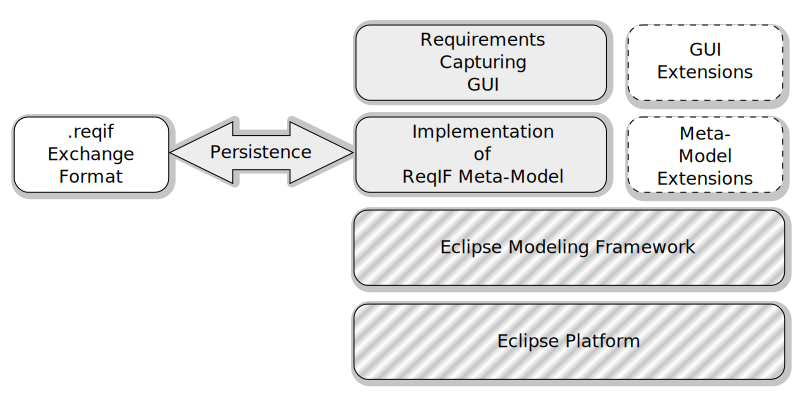
\includegraphics[width=\textwidth]{img/architecture.pdf}
	\end{center}
	\caption{High-level architecture of RMF}
	\label{fig:architecture}
\end{figure}

The GUI for capturing requirements is called ProR.  It operates directly on the ReqIF data model.  This is an advantage compared to existing requirements tools, where a transformation between ReqIF and the tool's data model is necessary.  Not all tools support all ReqIF features, therefore information may be lost in the process.  ProR at this time only supports the current version of ReqIF 1.0.1, not the older versions.

These contributions have their origins in research projects, where they are actively used. In particular, these research projects already produced extensions, demonstrating the value of the platform.  But ProR has reached a level of maturity that makes it fit for industrial use.  In particular, RMF has been used in the ProSTEP ReqIF Implementor Forum, a forum for tool vendors, to demonstrate interoperability of various requirements tools, including ProR \cite{prostep_if}.

\subsection{Extending RMF}

RMF is designed as a generic framework for requirements modeling, and the ProR GUI is designed as an extensible application.  It has been used and extended in various projects. Particularly relevant for openETCS, the Event-B evaluation used the Rodin extension of ProR to create a traceability of textual requirements to the Event-B benchmark \cite{event_b_benchmark}.

This is an important aspect of the project.  As we have seen in industry, heavy tailoring to the processes used and integration with other tools is what makes requirements tools successful.  By using Eclipse as the platform for this tool, we can provide integration with modeling tools like Rodin \cite{jastram_forms_2012} or Topcased \cite{topcase-JaGr2011}.  By providing a versatile extension point, the behavior of the application can be adapted to the process employed.

\section{ProR}
\label{pror}

ProR is the Graphical User Interface (GUI) or RMF.  ProR is available as a stand-alone application, and it can be integrated into existing Eclipse installations.  

The rest of this document describes how to actively work with ProR, and how to use certain features for the problem at hand.  A general overview of ProR will not be provided in this document, but many descriptions of the GUI are available \cite{RMF_Mark_Book_Jastram_2013, reqif_ObjektSpektrum_2013}.  

Further, the RMF website \cite{RMF} features a 15-minute video, demonstrating the most important features of the tool.  For readers not familiar with Eclipse and/or requirements tools, watching the video may be a good preparation for the next chapters.

%==============================================================================
\chapter{ProR Installation and Configuration}
%==============================================================================

This chapter is concerned with the installation and configuration of ProR.  The installation is straight forward, but configuring team support requires some attention.  This chapter is designed in a tutorial style, resulting in a running version of ProR, with the Benchmark project active and enabled for team work.

\section{Installing ProR}

ProR can be downloaded stand-alone, or installed into an existing application via its update site.  The download is a convenient option for non-technical people who just want to get started with ProR.  There are no special restriction for the update site version: ProR can be installed into any reasonably new Eclipse installation.  However, some care has to be taken in particular regarding compatibility of the modeling tools, if the host installation uses them as well.  Follow the following steps to install ProR:

\begin{description}

\item[Download ProR.]  The download URL is \url{http://eclipse.org/rmf/download.php}.  The benchmark has been performed with version 0.8.0.  Pick the correct file for your operating system.

\item[Unpack ProR.]  The downloaded file is a zip file, which needs to be unpacked in a new folder that you need to create.

\item[Launch ProR.] In the folder you will find a file named ``rmf-pror'' (possibly with the .exe extension).  You launch ProR by doubleclicking this file. \textbf{Tip:} It is convenient to create a shortcut to this file for launching.

\item[Pick a workspace.] Upon launching, you will be prompted for a workspace location.  The default is as good as any other. \textbf{Tip:} If you check ``Use this as default'' you won't be bothered with this dialog any more.

\item[Dismiss the Welcome Screen.] When launched for the first time, a welcome screen is shown.

\end{description}

\section{Team Support}

For openETCS, it is important to be able to work in a team setting.  Eclipse already provides a lot of the infrastructure for this.  However, an extension to ProR is available that automates a lot of the activities that are necessary in a team setting.  More importantly, this extension allow the comparing of requirements via the data model (instead of using XML files).  This makes it mutch easier to resolve conflicts, should they arise.

Team support is part of a free suite of extensions called ProR Esssentials.  While it is possible to install just individual components of this suite, we recommend to install all of them.  Follow the following steps to install ProR:

\begin{description}

\item[Select Help | Install new Software...] A dialog will open

\item[Set ``Work with:''.]  From the dropdown, select the entry ending in ``essentials''.

\item[Select ``ProR Essentials''.]  Once selected, complete the wizard.  There will be a warning that the software is not signed.

\item[Restart.] The wizard will give you the option to restart, please do it.

\item[Newsletter Subscription.] We hope that you will subscribe to the ProR newsletter, but this can be declined.

\end{description}

\section{Importing the Benchmark}

Now that team support is installed, it still has to be configured.  Team support uses Subversion.  As gitHub allows access via subversion, we can access all projects from gitHub.

\textbf{Tip:} Before proceeding please make sure you have your gitHub password ready.  You can proceed without it, but then you only have read acess.

\begin{description}
\item[File | Import...] This will open a dialog.
\item[Project from SVN.] In the folder SVN, select the option ``Project from SVN''
\item[Select a Connector.] This will trigger a new dialog.  There are many ways for giving Eclipse access to Subversion, broadly separated into native connectors (that use your locally installed Subversion) or connectors programmed in pure Java (not relying on any OS resources).  We recommend the second, specifically SVN Kit 1.7.10.  This will trigger an installation wizard, which you have to follow through and eventually restart ProR.
\item[Restart]
\item[Redo the previous steps.]  Du to the installation, you have to repeat the previous steps: File | Import... | Project from SVN.
\item[Provide the Project URL.] For the Benchmark, we use the Subversion-URL from gitHub, extended by the path to the project, which is \url{https://github.com/openETCS/model-evaluation/trunk/management/ProR_FormalMind/ProR_Benchmark}.  How the dialog is supposed to look is shown in Figure~\ref{fig:svn-config}.  Of course, you have to provide your own credentials.
\item[Complete the Wizard.]  Complete the wizards with all the given defaults.   \textbf{Tip:} Providing your gitHub credentials may trigger the secure storage.  This is an Eclipse-specific or OS-specific storage which will hold your gitHub password --- you can set any password, not (necessarily) the gitHub password.

\end{description}

With this, you have the Benchmark in your workspace, enabled for team work.

\begin{figure}[h!]
	\begin{center}
	\includegraphics[width=.8\textwidth]{img/svn-config.png}
	\end{center}
	\caption{Importing the Benchmark into ProR.}
	\label{fig:svn-config}
\end{figure}

%==============================================================================
\chapter{Benchmark}
%==============================================================================

This chapter describes the process of modeling the requirements with ProR and discusses various aspects of the modeling process.

\section{How to Model}

There are many ways to skin a cat.  This section discusses a number of general questions on how to go about modeling.

\subsection{Handling IDs}

It is best practice to give each element a user-readable ID.  Note that each ReqIF element has an internal unique ID that never changes, but that is not meant to be user readable.  Considering that most elements already have an ID in the ERA document, we decide to keep those.

A plugin for ProR exists (a so-called Presentation) that automatically generates read-only user-readable IDs.  This would result in labels like ``REQ-1''.  This mechanism should be employed when creating new elements.  In this situation, however, they don't seem to make sense.

\subsection{Plain Text or Rich Text?}

The ReqIF standard, and as a consequence ProR, support rich text (formatted text).  While formatted text may seem more attractive (especially, as the ERA documents are available as formatted Word documents), we reject it for §6.  The main reason is that formatted text is much harder to process by other tools (e.g. constraining the requirements text with a DSL).

However, to demonstrate that it is possible, we used rich text for modeling sections of §3.

It is possible to mix formatted and plain text.  For instance, text that exists for information only could be formatted, while the actual requirements are kept in plain text.

Limited formatting could also be applied to plain text, by giving certain datatypes specific formatting.  We chose this solution for §6 and use it to format headlines.

\textbf{Note:} To use rich text, ProR requires at least Java 7 from Oracle (not OpenJDK).

\subsection{Inconsistencies in the Spec}

There were a number of problems with the Word-based specification used.  Specifically:

\begin{itemize}

\item The document was in change mode, resulting in strange emtpy blocks (e.g. 6.6.2.1.2 -- 6.6.2.1.7, followed by an empty table).

\item Some headlines did not have a section number, e.g. ``Exceptions to chapter 4''.  However, the correct section number could not be inferred.

\item Some headlines did not have a section number, but allowed the correct number to be inferred, e.g. ``General'' between 6.6.3 and 6.6.3.1.1.

\item However, as all the numbering is generated by Word, it should be considered fragile.

\end{itemize}

\subsection{Tables}
\label{sec:tables}

The document contains a number of tables, and it's not clear what the best option for modeling them is.  ReqIF supports tables, with each table cell being one SpecObject.  However, ProR currently does not support the visualization of such tables (they can be created and read, but will not be shown in a table structure).

However, even if this feature were implemented in a user-friendly way, using it would bypass the rich type system that ReqIF provides.  Instead, we created a dedicated SpecType for each table row.  The description would be used as the label, while there would be table-specific attributes of the proper type (constraint integers, enumerations, etc.).  This would also make further automated processing much easier.  The downside is, that not all table columns are visible.  To see all values in the Properties View, a row must be selected.  Of course, the tabular view could be extended to show all columns with a few clicks.  But this would result in showing columns that are used in only a few rows.

The worst option would be to use rich text, to put a (XHTML) table in one SpecObject.

Other options may be available.  But it is clear that the constrains imposed by the word processor do not have to be transferred to ProR.

Figure~\ref{fig:packet-action-table} shows how this looks in practice.  The package action table (after 6.6.3.1.5 in the document) has four columns.  Two of these have been mapped to the visual columns \emph{ID} and \emph{Description}.  The other two (\emph{Operated system version number X = 1} and \emph{2}) are only visible in the properties view.  Not visible in the screenshot is the fact that the ID is restricted to the range 0--255, and that the entries for the last two columns are selected from a dropdown.

Some of the entries have footnotes.  These have been modeled as links.  The link targets can be seen at the bottom, and the right column shows that select row (Packet Number 51) has two outgoing links.  The link targets don't have to be visible: Links can be expanded, and by selecting an individual link, the properties of the target will be shown in the properties view.

\begin{figure}
	\begin{center}
	\includegraphics[width=.8\textwidth]{img/packet-action-table.png}
	\end{center}
	\caption{Representing the Package Action Table in ProR, using attributes instead of columns.}
	\label{fig:packet-action-table}
\end{figure}

\section{Rich Text and References}

As mentioned earlier, parts of §3 have been modeled using rich text.  This is shown in Figure~\ref{fig:xhtml-and-links}, demonstrating some of the rich text capabilities.  For instance, bullet lists, bold and strike-through are supported.

\begin{figure}
	\begin{center}
	\includegraphics[width=\textwidth]{img/xhtml-and-links.png}
	\end{center}
	\caption{Using rich text and SpecRelations to provide references.}
	\label{fig:xhtml-and-links}
\end{figure}

The figure also shows that the original text has been modified, with new text inserted and removed text stroked out (this has been done manually, not automatically).  This has been done mainly to remove references that have been inserted into the original document as plain text.  Doing this is highly fragile: Inserting another paragraph in Word would change the subsequent numbering, leaving an incorrect reference\footnote{Incidentally, Word does in fact support cross-referencing, which would have solved at least this problem.  Why this has not been used for a document like this is beyond me.}.  The reference has been replaced with a SpecRelation.  In the figure, the two references to 3.12.3.4.2 and .3 have been expanded.  The description text of those links is empty, but by giving the SpecRelation attributes, some information could be entered here.

\section{Traceability}

Traceability is a crucial feature for openETCS.  Traces in ProR are modeled using SpecRelations.  These have already been put to use for linking footnotes, as described in Section~\ref{sec:tables}.  However, that use does not show the full potential of traces.

For this case study, we show how traceability between §6 and §3 can be realized.  The following requirement will be used:

\includegraphics[width=\textwidth]{img/R-66211.png}

In contrast to the SpecRelations used earlier, a typed SpecRelation will be used this time to:

\begin{itemize}
\item Be able to annotate the trace with a description.
\item To track whether the source or target of the SpecRelation has changed (for change management).
\end{itemize}

Change management can be realized with the ``Linkmanagement Presentation'', an extension from the ProR Essentials.  To use it, a new SpecType for SpecRelatons has to be created with two boolean flags (for source and target, respectively).  this is done via \emph{ProR | Datatype Configuration...}  Next, the presentation has to be added (via \emph{ProR | Presentation Configuration...}).

Once this is set up, a link between the two elements (6.6.2.1.1 and 3.12.3.4.7.2) can be established.  There are various ways to acomplish this.  The easiest is to use the element's context menu to select \emph{Initiate Linking}, and then to select the target element, selecting \emph{} from the context menu, using the SpecType we previously created.

\begin{figure}
	\begin{center}
	\includegraphics[width=\textwidth]{img/link-target-selected.png}
	\end{center}
	\caption{Showing the link target in the Properties View.}
	\label{fig:link-target-selected}
\end{figure}

As a result, element 6.6.2.1.1 has now an outgoing SpecRelation, which can be expanded.  Selecting the SpecRelation's row will show the attributes of that SpecRelation.  However, selecting the last cell in that row (the \emph{Link} column), the target element will be shown in the Properties View, as shown in Figure~\ref{fig:link-target-selected}.

Now the change can be applied by updating element 3.12.3.4.7.2, which can be done directly in the Properties View.  For good measure, some information on what has been done can be written in the description attribute of the SpecRelation.  Figure~\ref{fig:link-target-changed} shows this, but this time with the SpecRelation selected.  Note that the SpecRelation's description text is shown both in the main editor, as well as in the Properties View.  Also note that the ``Target'' Attribute in the Properties View now shows a yellow warning triangle.  This has been set by the Linkmanagement Presentation: It noticed that the target element had changed and set the flag correspondingly.  Users can reset it by doublecklicking it, indicating that they verified the trace.  The opposite is possible too: traces can be marked manually for inspection.

\begin{figure}
	\begin{center}
	\includegraphics[width=\textwidth]{img/link-target-changed.png}
	\end{center}
	\caption{Showing the link target in the Properties View.}
	\label{fig:link-target-changed}
\end{figure} 

\section{Traceability to EMF-based Models}

Integrating ProR with other EMF tools is out of the scope of this document.  As mentioned before, some of this has already been explored in the Event-B benchmark \cite{event_b_benchmark}, e.g. in Figure~13 in that report.

Integration with existing EMF models can take place on two levels, both which are shown in Figure~\ref{fig:proxy-1}, which has been taken from \cite{integrate-models}:

\begin{figure}
	\begin{center}
	\includegraphics[width=0.8\textwidth]{img/proxy-1.png}
	\end{center}
	\caption[Seamless integration of models and requirements]{Showing how models and requirements can be integrated seamlessly. The first row shows color highlighting in the requirements text.  The colored symbols are defined in the associated Event-B model.  The second row shows an element from the Event-B model, which is referenced and therefore never outdated.}
	\label{fig:proxy-1}
\end{figure} 

\begin{description}
\item[Linking to model elements.]  ProR supports a mechanism to create proxy elements that retrieve the content of other model elements and renders them in an appropriate fashion directly in the specification.
\item[Color highlighting of model element names.] It is also possible to use color highlighting in the requirements text to identify symbols that are defined in another model.  Currently this has only been realized using plain text attributes, as interfering with the formatting of rich text attributes is tricky.
\end{description}

\section{Reporting}

Reporting capabilities are currently limited to converting a Specification to HTML.  This is realized by selecting the editor containing the Specification to be exported and to initiate \emph{File | Print...}.  ProR will open a Web Browser with the exported Specification.

A Master student at the University of Düsseldorf is implementing advanced reporting as part of his thesis.  This work is expected to be available in the open source by the end of the year.

\section{Using Team Support}

The team support from the ProR Essentials makes the most often used team actions available via the project's context menu (in the \emph{ProR} submenu).  The same, and more advanced actions are in the \emph{Team} context menu of the project.

The team support offers more features, which are described as follows.  However, these features seem to be broken in 0.8.0.  We plan to fix them with the next version of ProR Essentials, expected in October 2013.

Team support can be used to browse the history of the project or individual files (\emph{Team | Show History}).  Differences between files can be inspected by selecting two files and picking \emph{Compare with Each Other} from the context menu (currently broken).  Rather than comparing the XML files, the two model trees will be compared, as shown in Figure~\ref{fig:model-diff}.  This feature is described in detail in \cite{essentials_diff}.  A corresponding model viewer can be used to perform merges in the case of conflicts.

\begin{figure}
	\begin{center}
	\includegraphics[width=.8\textwidth]{img/model-diff.png}
	\end{center}
	\caption[Comparing Models with ProR Essentials Diff.]{Comparing Models with ProR Essentials Diff.  Rather than having a textual diff of the XML, the tool compares the model representation of the two versions.  The structural differences are shown in a tree (1), while the actual changes can be compared graphically next to each other (3), with the ability to look at the actual properties (4).  Step by step navigation through the changes is possible (2).}
	\label{fig:model-diff}
\end{figure}

In addition to this, the team extension provides a number of convenience features (currently broken):

\begin{description}
\item[Auto-Add.] New files in the project will automatically be added to version control.  Currently, this has to be done by hand (can be done as part of the commit process).
\item[Auto-Update.] Users can elect to automatically run a subversion update upon opening a project.  This ensures that they will always have the latest version of the requirements, minimizing the risk of conflicts.
\item[Auto-Commit.] Users can elect to automatically run a subversion commit upon closing the project.  This will ensure that changes are pushed to the server as soon as possible, minimizing the risk of conflicts.
\end{description}

\section{Performance}
\label{sec:performance}

Due to time constraints, only a small number of requirements have been modeled.  Therefore, this benchmark is not adequate to evaluate the performance of the tool.

However, ProR has been shown to handle thousands of requirements easily, which should be sufficient for fulfilling the needs of the openETCS project.

Performance is a crucial issue in the car industry, where ProR is already deployed.  Here, users often have to deal with tens of thousands of requirements, and the goal of the project is to support that with an acceptable performance.  Therefore, performance is expected to improve over time even more.

Last, a progress bar is shown upon opening a file, giving the user an indication on how long this will take.  Once open, the performance is usually fast.  Further, the progress bar slows the opening of a file down for small files, but not for big ones (this is a bug).  Thus, the speed of opening a small file should not be taken as an indication on how much longer it would take to open a big one.

\section{Issues to be Resolved}

We believe that this benchmark demonstrates that many of the features required for requirements management, engineering and traceability are found in ProR.  Nevertheless, a few issues that need to be resolve have been identified:

\begin{description}

\item[Open Source.] ProR is open source, and licenced under EPL, which is EUPL compatible.  However, the components from the ProR Essentials are closed source, belonging to Formal Mind.  If ProR is adopted for openETCS, we will open source those components that are used by openETCS.

\item[Traceability to ERA documents.]  The ERA documents are currently available as Microsoft Word documents.  We recommend the development of an importer that will allow to reimport those word documents without losing traceability.

\item[Handling Tables.]  The ReqIF standard supports a scheme for managing tabular data, where each cell in the table is an atomic element.  ProR supports this, but the representation is not user friendly.  We recommend implementing a better representation for ReqIF tables.

\item[Team Integration.]  The current implementation hints at what is possible, but some features that were implemented before are currently broken.  These will be fixed in the next update, expected in October 2013.

\end{description}

%==============================================================================
\chapter{Conclusion}
%==============================================================================

We believe that we have demonstrated that professional requirements management and traceability is possible with ProR, and that traceability in EMF-based models can be realized with reasonable effort.  As important ProR is a tool that fulfills a number of requirements that are essential for openETCS, including being open source and being based on Eclipse and EMF.

This report covers essential features for openETCS, including:

\begin{itemize}
\item Version control
\item Atomic requirements with arbitrary typed attributes
\item Plain text and rich text requirements
\item Organization of multiple documents
\item Traceability with attributed traces
\item Change Management
\item Integration with other EMF-based tools
\end{itemize}

Last, as ProR is based on the well-documented international ReqIF standard, integration with other tools is possible and relatively easy.

%\nocite{*}

\bibliographystyle{plain}
\bibliography{literature}

\appendix

% \chapter{Aenean imperdiet}

% \lipsum[12-16]


%===================================================
%Do NOT change anything below this line

\end{document}
